%File: formatting-instructions-latex-2024.tex
%release 2024.0
\documentclass[letterpaper]{article} % DO NOT CHANGE THIS
\usepackage{aaai24}  % DO NOT CHANGE THIS
\usepackage{times}  % DO NOT CHANGE THIS
\usepackage{helvet}  % DO NOT CHANGE THIS
\usepackage{courier}  % DO NOT CHANGE THIS
\usepackage[hyphens]{url}  % DO NOT CHANGE THIS
\usepackage{graphicx} % DO NOT CHANGE THIS
\urlstyle{rm} % DO NOT CHANGE THIS
\def\UrlFont{\rm}  % DO NOT CHANGE THIS
\usepackage{natbib}  % DO NOT CHANGE THIS AND DO NOT ADD ANY OPTIONS TO IT
\usepackage{caption} % DO NOT CHANGE THIS AND DO NOT ADD ANY OPTIONS TO IT
\frenchspacing  % DO NOT CHANGE THIS
\setlength{\pdfpagewidth}{8.5in}  % DO NOT CHANGE THIS
\setlength{\pdfpageheight}{11in}  % DO NOT CHANGE THIS
%
% These are recommended to typeset algorithms but not required. See the subsubsection on algorithms. Remove them if you don't have algorithms in your paper.
\usepackage{algorithm}
\usepackage{algorithmic}
\usepackage{bm}
%
% These are are recommended to typeset listings but not required. See the subsubsection on listing. Remove this block if you don't have listings in your paper.
\usepackage{newfloat}
\usepackage{listings}
\DeclareCaptionStyle{ruled}{labelfont=normalfont,labelsep=colon,strut=off} % DO NOT CHANGE THIS
\lstset{%
	basicstyle={\footnotesize\ttfamily},% footnotesize acceptable for monospace
	numbers=left,numberstyle=\footnotesize,xleftmargin=2em,% show line numbers, remove this entire line if you don't want the numbers.
	aboveskip=0pt,belowskip=0pt,%
	showstringspaces=false,tabsize=2,breaklines=true}
\floatstyle{ruled}
\newfloat{listing}{tb}{lst}{}
\floatname{listing}{Listing}
%
% Keep the \pdfinfo as shown here. There's no need
% for you to add the /Title and /Author tags.
\pdfinfo{
/TemplateVersion (2024.1)
}

% DISALLOWED PACKAGES
% \usepackage{authblk} -- This package is specifically forbidden
% \usepackage{balance} -- This package is specifically forbidden
% \usepackage{color (if used in text)
% \usepackage{CJK} -- This package is specifically forbidden
% \usepackage{float} -- This package is specifically forbidden
% \usepackage{flushend} -- This package is specifically forbidden
% \usepackage{fontenc} -- This package is specifically forbidden
% \usepackage{fullpage} -- This package is specifically forbidden
% \usepackage{geometry} -- This package is specifically forbidden
% \usepackage{grffile} -- This package is specifically forbidden
% \usepackage{hyperref} -- This package is specifically forbidden
% \usepackage{navigator} -- This package is specifically forbidden
% (or any other package that embeds links such as navigator or hyperref)
% \indentfirst} -- This package is specifically forbidden
% \layout} -- This package is specifically forbidden
% \multicol} -- This package is specifically forbidden
% \nameref} -- This package is specifically forbidden
% \usepackage{savetrees} -- This package is specifically forbidden
% \usepackage{setspace} -- This package is specifically forbidden
% \usepackage{stfloats} -- This package is specifically forbidden
% \usepackage{tabu} -- This package is specifically forbidden
% \usepackage{titlesec} -- This package is specifically forbidden
% \usepackage{tocbibind} -- This package is specifically forbidden
% \usepackage{ulem} -- This package is specifically forbidden
% \usepackage{wrapfig} -- This package is specifically forbidden
% DISALLOWED COMMANDS
% \nocopyright -- Your paper will not be published if you use this command
% \addtolength -- This command may not be used
% \balance -- This command may not be used
% \baselinestretch -- Your paper will not be published if you use this command
% \clearpage -- No page breaks of any kind may be used for the final version of your paper
% \columnsep -- This command may not be used
% \newpage -- No page breaks of any kind may be used for the final version of your paper
% \pagebreak -- No page breaks of any kind may be used for the final version of your paperr
% \pagestyle -- This command may not be used
% \tiny -- This is not an acceptable font size.
% \vspace{- -- No negative value may be used in proximity of a caption, figure, table, section, subsection, subsubsection, or reference
% \vskip{- -- No negative value may be used to alter spacing above or below a caption, figure, table, section, subsection, subsubsection, or reference

\setcounter{secnumdepth}{2} %May be changed to 1 or 2 if section numbers are desired.

% The file aaai24.sty is the style file for AAAI Press
% proceedings, working notes, and technical reports.
%

% Title

% Your title must be in mixed case, not sentence case.
% That means all verbs (including short verbs like be, is, using,and go),
% nouns, adverbs, adjectives should be capitalized, including both words in hyphenated terms, while
% articles, conjunctions, and prepositions are lower case unless they
% directly follow a colon or long dash
\title{Supplementary for Progressive Painterly Image Harmonization from Low-level Styles to High-level Styles}
\author{
    Li Niu\thanks{Corresponding author.},
    Yan Hong, 
    Junyan Cao, 
    Liqing Zhang 
    \\
}
\affiliations{
    %Afiliations
    MoE Key Lab of Artificial Intelligence, Shanghai Jiao Tong University\\
    % If you have multiple authors and multiple affiliations
    % use superscripts in text and roman font to identify them.
    % For example,

    % Sunil Issar, \textsuperscript{\rm 2}
    % J. Scott Penberthy, \textsuperscript{\rm 3}
    % George Ferguson,\textsuperscript{\rm 4}
    % Hans Guesgen, \textsuperscript{\rm 5}.
    % Note that the comma should be placed BEFORE the superscript for optimum readability

    % email address must be in roman text type, not monospace or sans serif
    \{ustcnewly, hy2628982280, joy\_c1, lqzhang\}@sjtu.edu.cn
%
% See more examples next
}
%Example, Single Author, ->> remove \iffalse,\fi and place them surrounding AAAI title to use it
\iffalse
\title{My Publication Title --- Single Author}
\author {
    Author Name
}
\affiliations{
    Affiliation\\
    Affiliation Line 2\\
    name@example.com
}
\fi

\iffalse
%Example, Multiple Authors, ->> remove \iffalse,\fi and place them surrounding AAAI title to use it
\title{My Publication Title --- Multiple Authors}
\author {
    % Authors
    First Author Name\textsuperscript{\rm 1,\rm 2},
    Second Author Name\textsuperscript{\rm 2},
    Third Author Name\textsuperscript{\rm 1}
}
\affiliations {
    % Affiliations
    \textsuperscript{\rm 1}Affiliation 1\\
    \textsuperscript{\rm 2}Affiliation 2\\
    firstAuthor@affiliation1.com, secondAuthor@affilation2.com, thirdAuthor@affiliation1.com
}
\fi


% REMOVE THIS: bibentry
% This is only needed to show inline citations in the guidelines document. You should not need it and can safely delete it.
\usepackage{bibentry}
% END REMOVE bibentry

\begin{document}

\maketitle

In this document, we provide additional materials to support our main paper. 
In Section~\ref{sec:exit_stage_annotation}, we provide the details and examples for annotated exit stages in the training set. In Section~\ref{sec:visualization}, we provide more visual comparison with baseline methods. In Section~\ref{sec:failure_case}, we discuss the failure cases of our method. 


\section{Exit Stage Annotation} \label{sec:exit_stage_annotation}

As introduced in the main paper (Section 3.2 and 4.2 in the main paper),  we randomly select $5000$ composite images in the training set and get their harmonized results from four stages. Then, we ask human annotators to manually select the exit stage for each composite image, in which the exit stage means the earliest stage with satisfactory harmonized output. 
In detail, if the result of one stage is significantly better than the others, they choose this stage as the exit stage. Otherwise, they choose the earliest one from multiple comparable stages. 
Considering the subjectiveness of this annotation task, we ask $50$ human annotators to annotate each composite image and decide the ground-truth exit stage according to major voting, that is, we choose the stage selected by most annotators as the exit stage. The percentages that four stages are annotated as the exit stage are $2.1\%$, $22.3\%$, $47.4\%$, and $28.2\%$ respectively. Overall, the outputs from late stages (\emph{e.g.}, 3, 4) are better than those from early stages (\emph{e.g.}, 1, 2), because the outputs from late stages are usually more sufficiently harmonized in terms of high-level styles. 

In Figure \ref{fig:exit_stages_train}, we show several examples of composite images and their harmonized results from four stages. We mark the annotated exit stages in red bounding boxes. 
As shown in Figure~\ref{fig:exit_stages_train}, in row 1-2, the results from the first three stages are not sufficiently harmonized, so the last stage is annotated as the exit stage. In row 3-4,  the results from the first two stages are already satisfactory, so the first stage or the second stage are annotated as the exit stages. In row 5-7, the results from the last stage have undesired artifacts (row 5) or distorted content structure (row 6-7), so the stages before the artifacts or distortion appear are annotated as the exit stages. Based on the above observations, our designed early-exit strategy is reasonable because different composite images should exit the network from different stages. Our annotated exit stages on the training set could provide effective supervision for learning to decide the exit stage automatically. 

\begin{figure}[t]
\centering
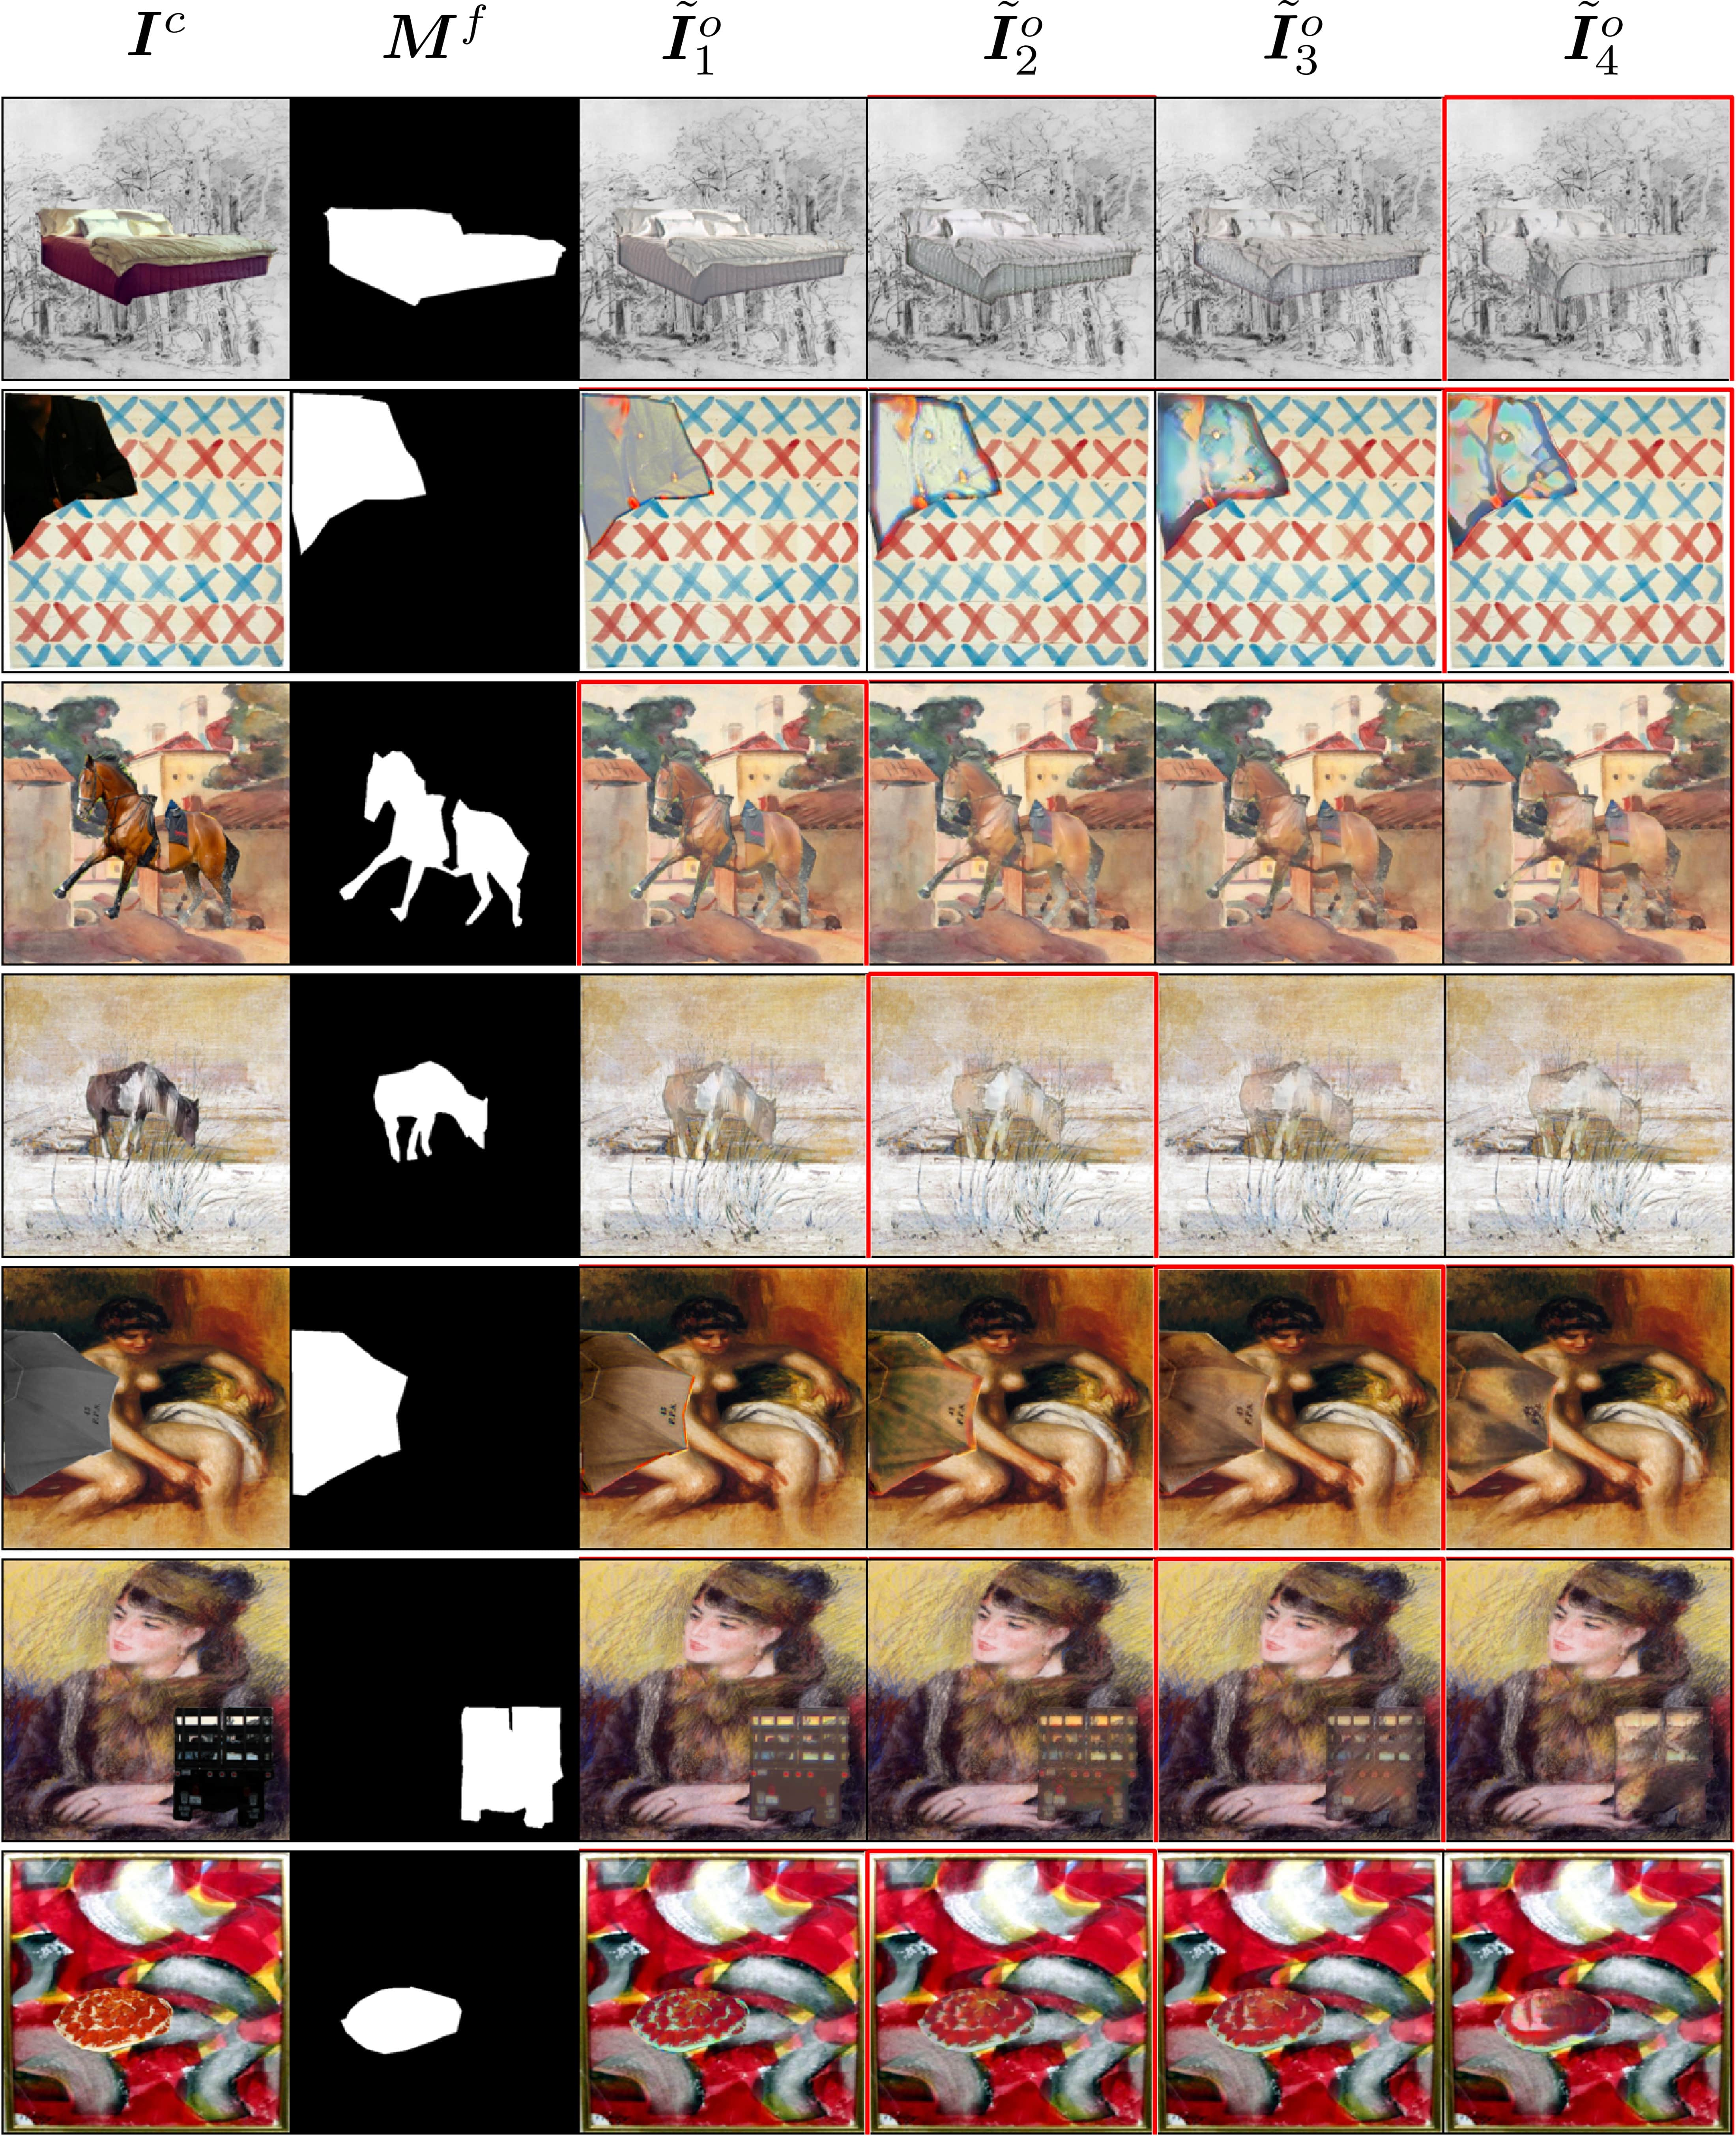
\includegraphics[width=0.99\linewidth]{figures/exit_stages_train.jpg}
\caption{From left to right, we show the composite image, composite mask, the harmonized results from four stages in the training set. The annotated exit stages are marked with red bounding boxes.}
\label{fig:exit_stages_train}
\end{figure}


\begin{figure}[t]
\centering

\includegraphics[width=0.85\linewidth]{figures/failure_cases.jpg}
\caption{Two example failure cases of our ProPIH.}
\label{fig:failure_cases}
\end{figure}

\begin{figure*}[t]
\centering
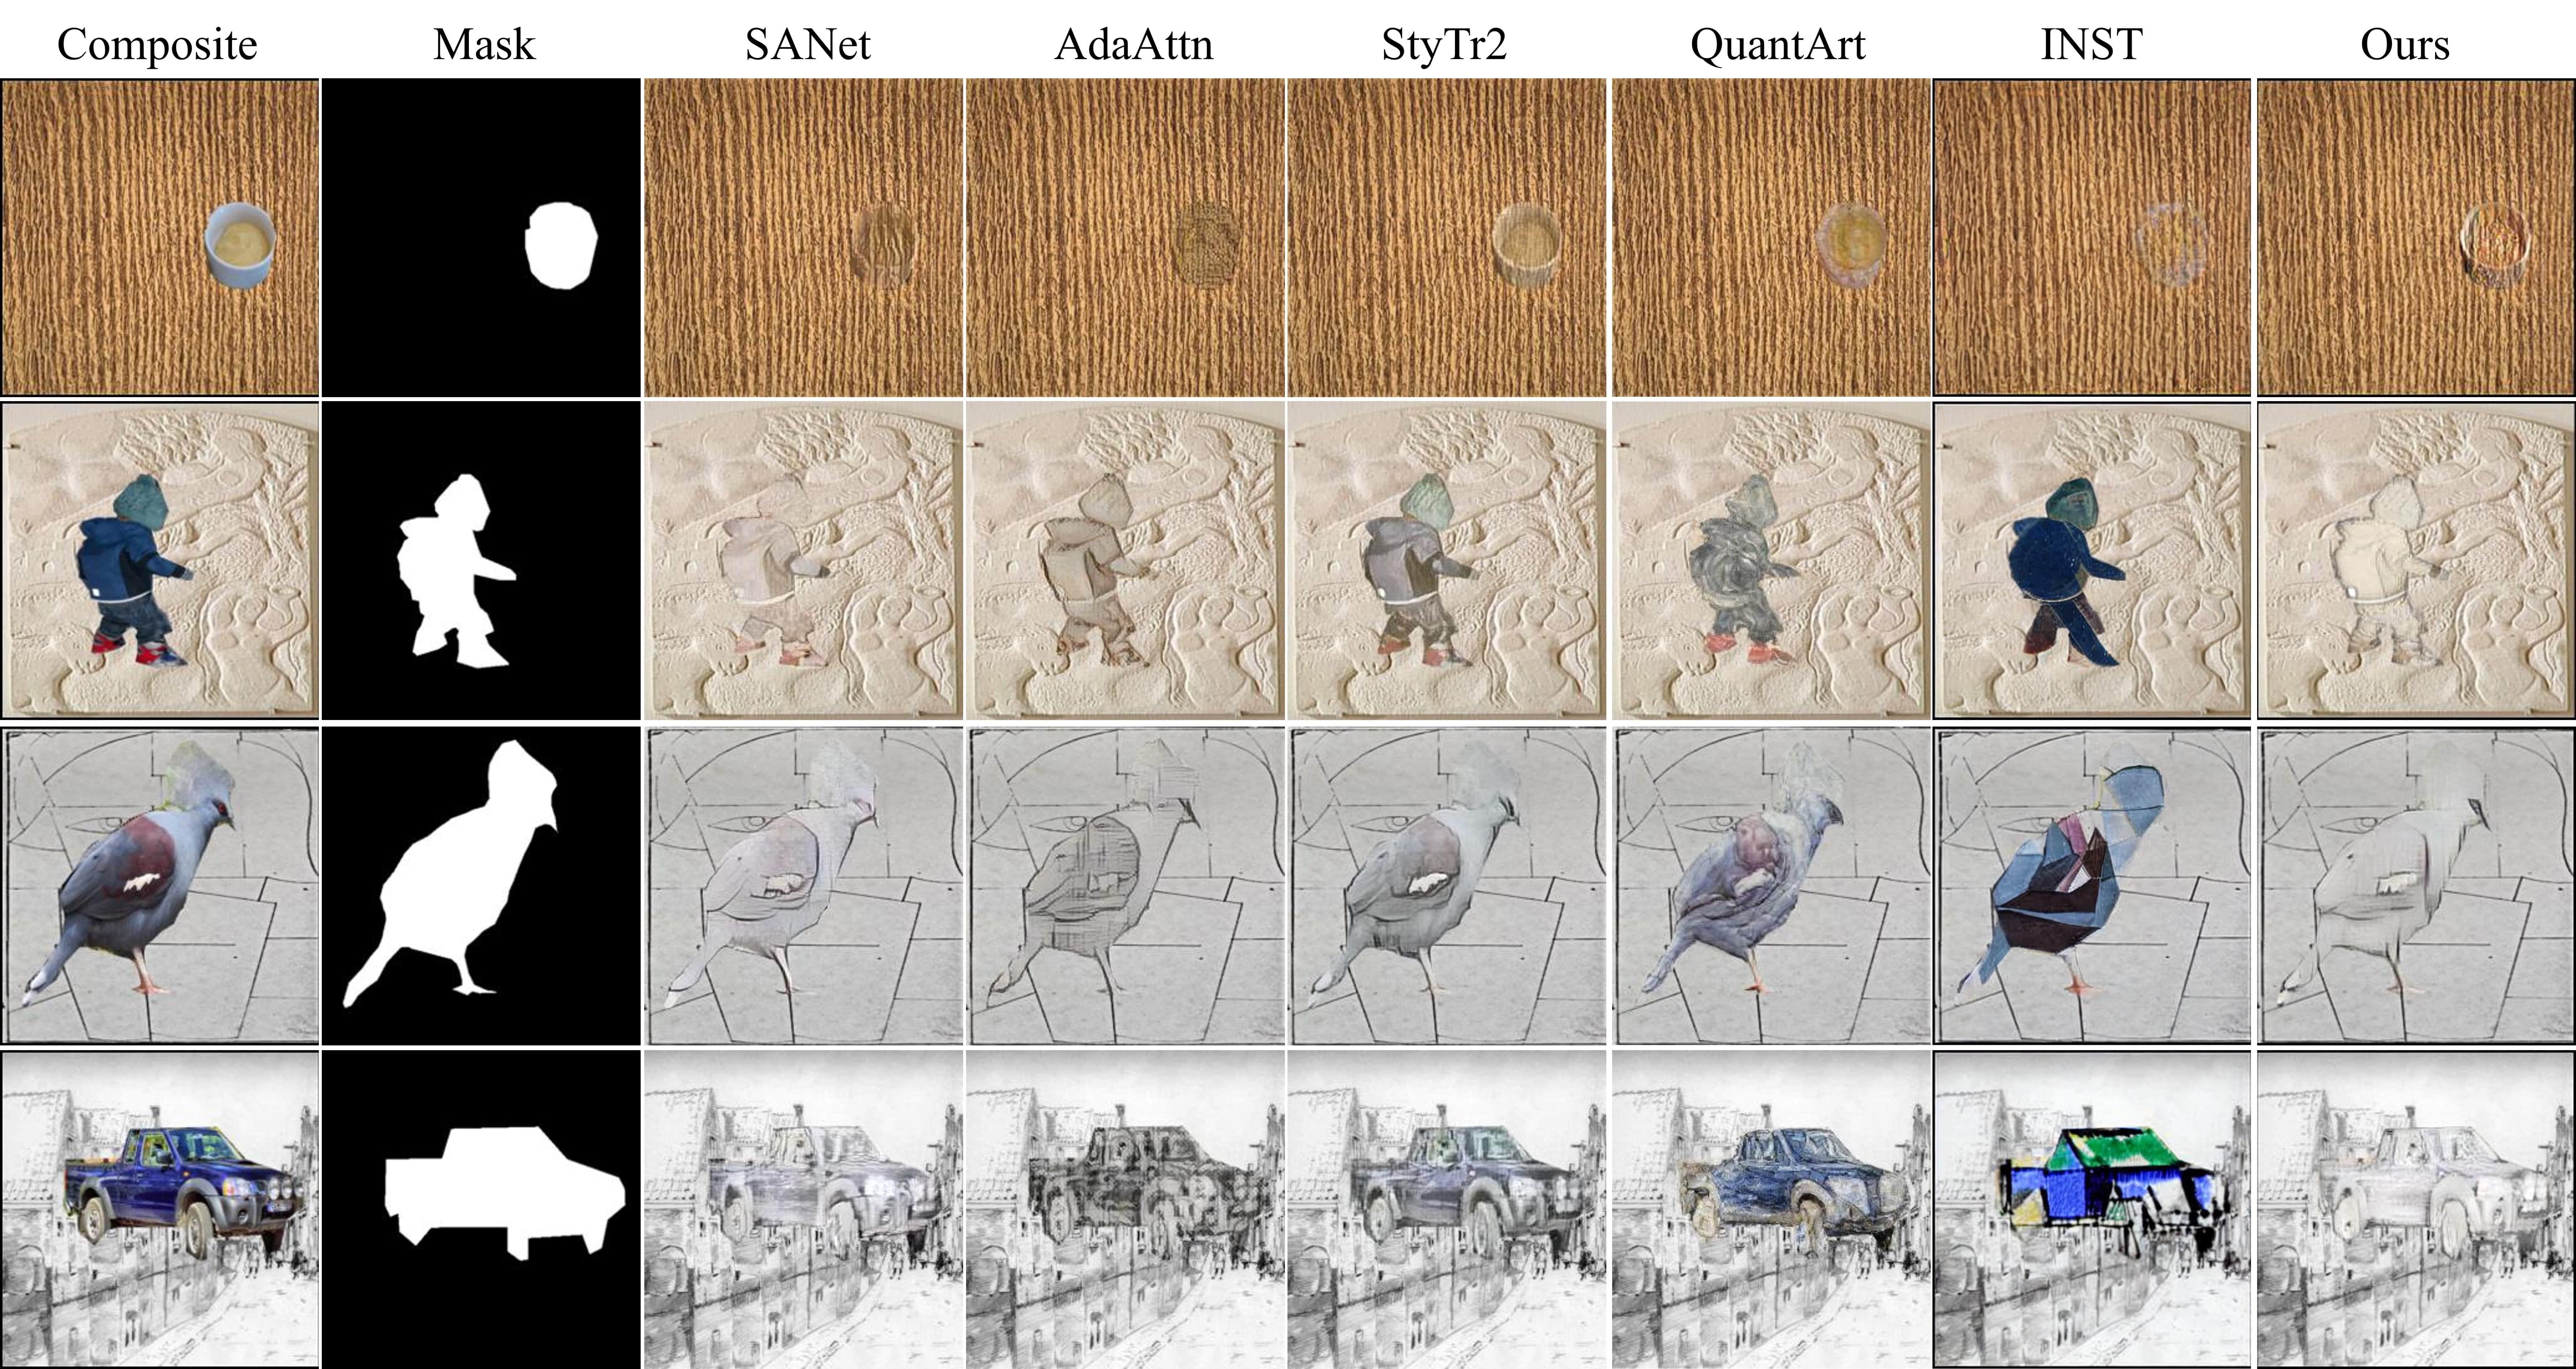
\includegraphics[width=0.99\linewidth]{figures/style_transfer_baselines_supp.jpg}
\caption{From left to right, we show the composite image, composite foreground mask, the harmonized results of  SANet~\cite{park2019arbitrary}, AdaAttN~\cite{liu2021adaattn}, StyTr2~\cite{deng2022stytr2}, QuantArt~\cite{quantart}, INST~\cite{inst}, and our ProPIH.}
\label{fig:style_transfer_baseline_supp}
\end{figure*}


\begin{figure*}[t]
\centering
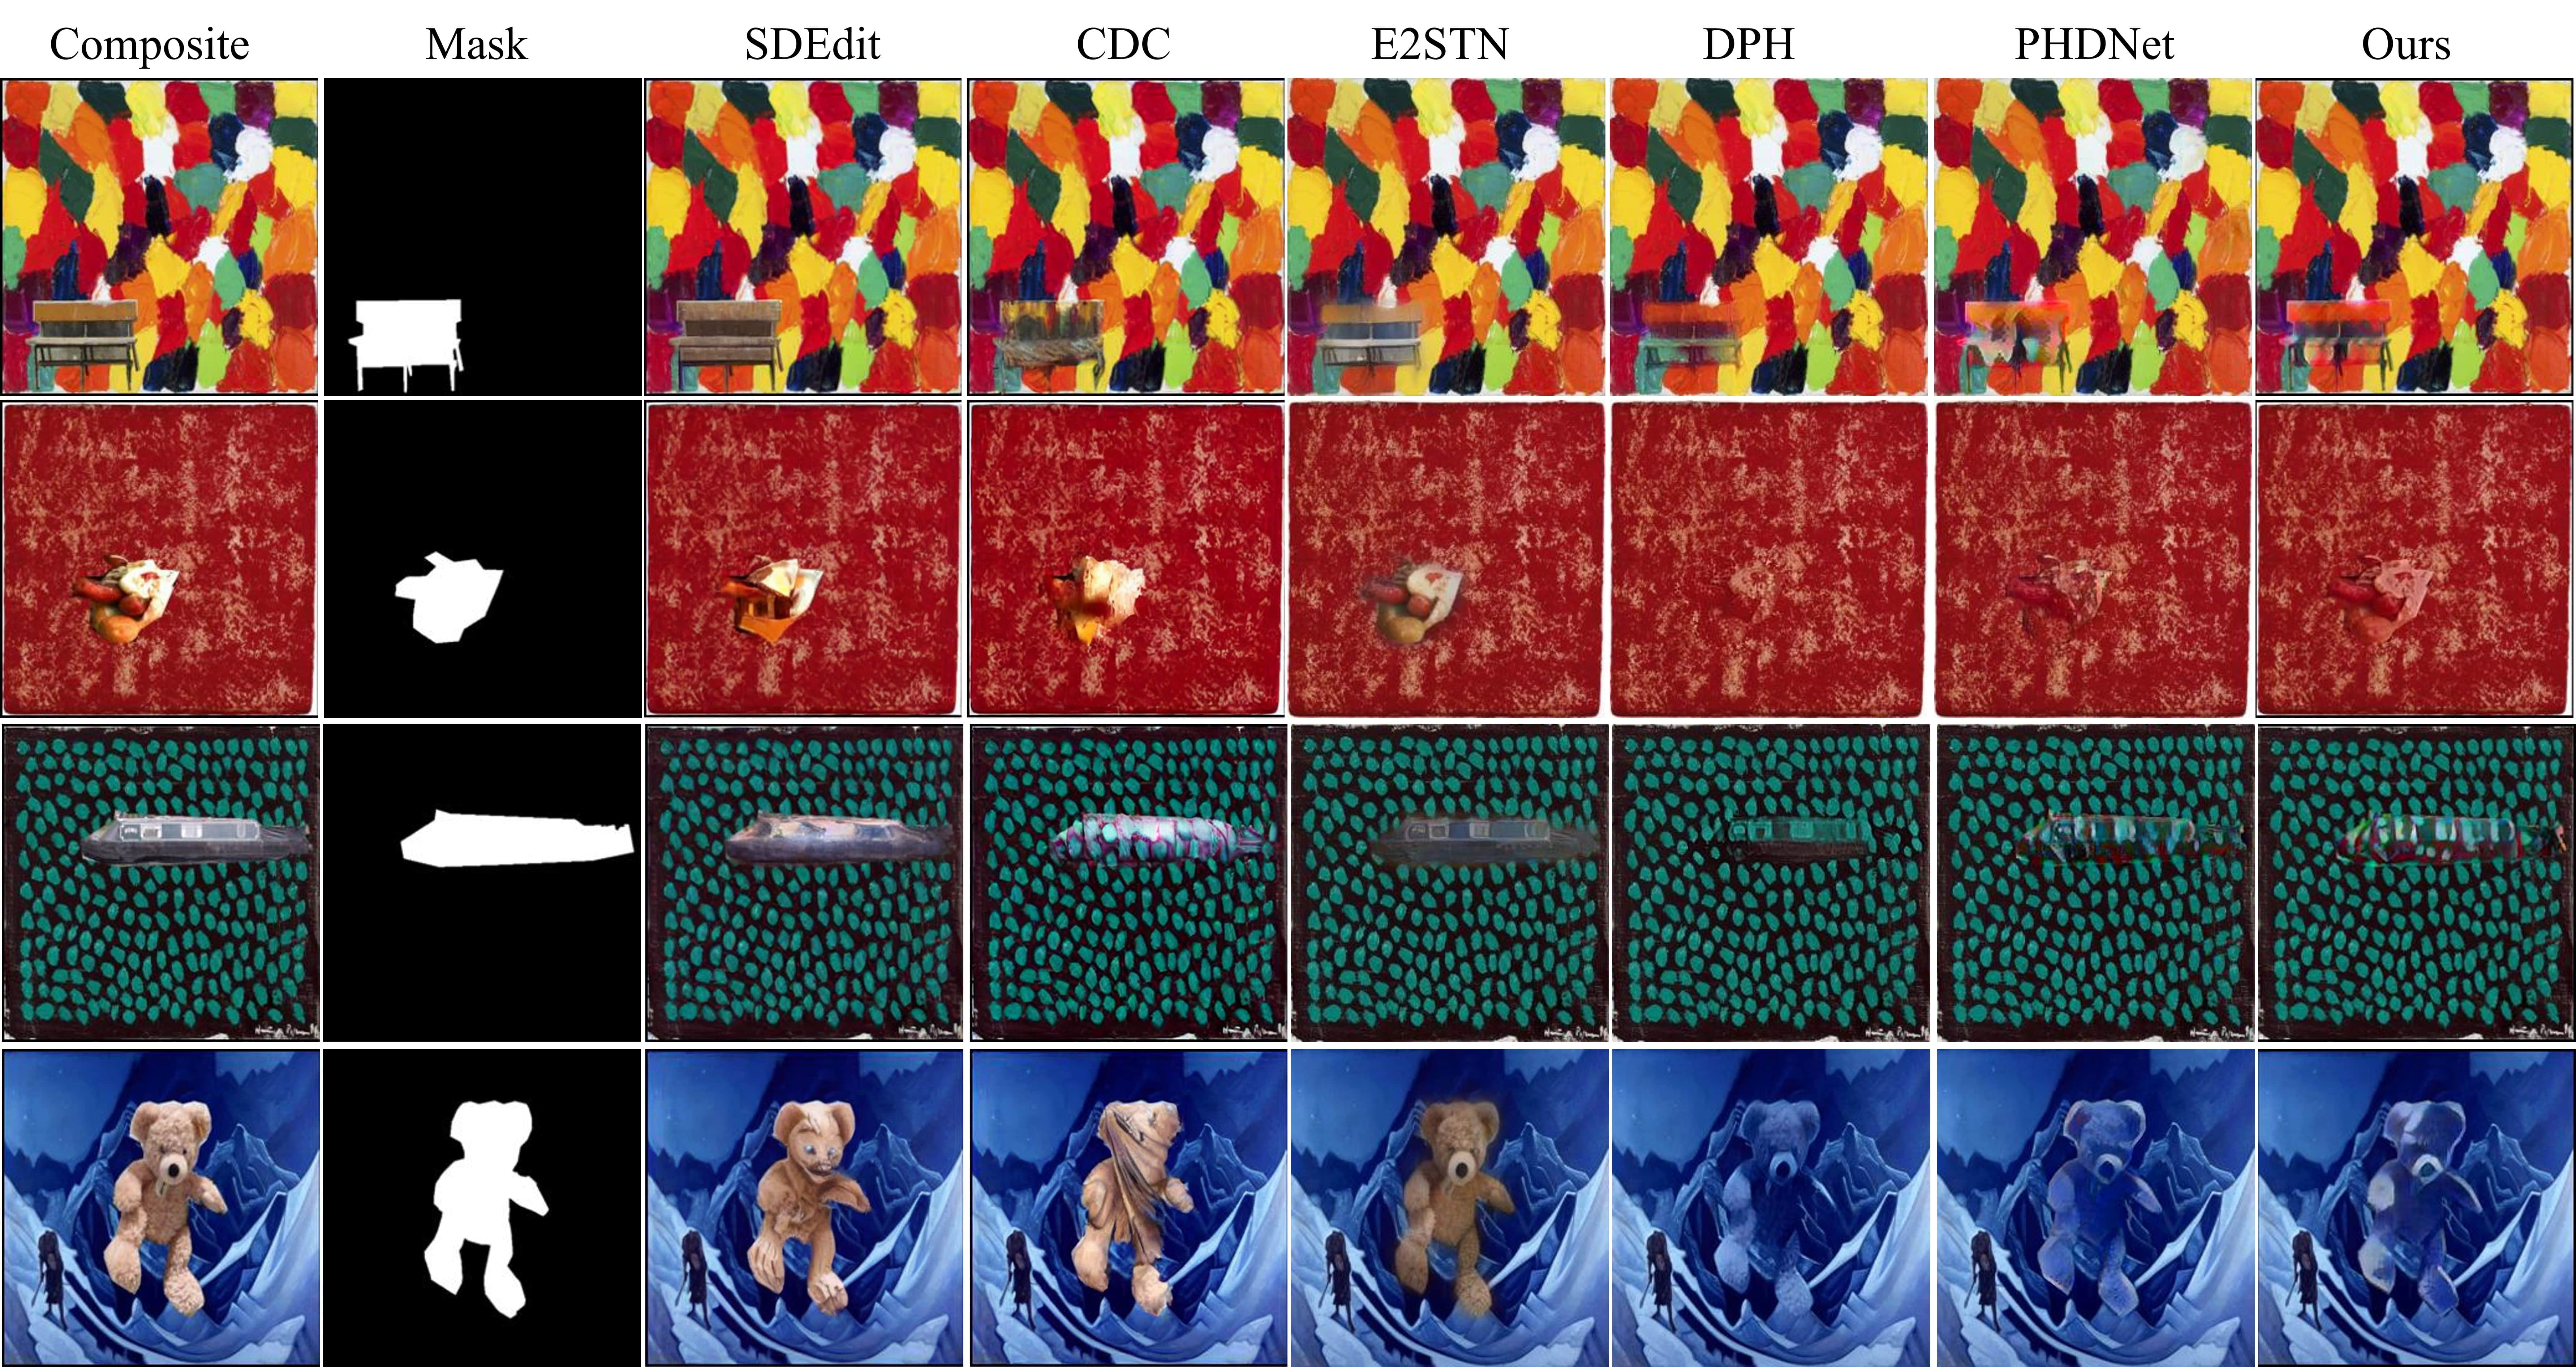
\includegraphics[width=0.99\linewidth]{figures/painterly_harmonization_baselines_supp.jpg}
\caption{From left to right, we show the composite image, composite foreground mask, the harmonized results of SDEdit~\cite{sdedit}, CDC~\cite{cdc}, E2STN~\cite{peng2019element}, DPH~\cite{luan2018deep}, PHDNet~\cite{cao2022painterly}, and our ProPIH.}
\label{fig:painterly_harmonization_baseline_supp}
\end{figure*}




\section{More Visualization Results} \label{sec:visualization}

In Section 4.3 in the main paper, we compare with two groups of baselines. The first group is artistic style transfer baselines: SANet~\cite{park2019arbitrary}, AdaAttN~\cite{liu2021adaattn},  StyTr2~\cite{deng2022stytr2}, QuantArt~\cite{quantart}, INST~\cite{inst}. 
The second group is painterly image harmonization baselines: SDEdit~\cite{sdedit}, CDC~\cite{cdc}, DPH~\cite{luan2018deep}, E2STN~\cite{peng2019element}, PHDNet~\cite{cao2022painterly}. In this section, we provide more comparison results with these two groups of baselines. 

We show the comparison with the first group of baselines in Figure \ref{fig:style_transfer_baseline_supp}. The baselines tend to insufficiently or incorrectly stylize the foreground objects, so that the foreground colors/textures are apparently inconsistent with the background colors/textures (\emph{e.g.}, the boy in row 2, the car in row 4). In contrast, our stylized foregrounds are more compatible with the backgrounds and naturally embedded into the backgrounds.

We show the comparison with the second group of baselines in Figure \ref{fig:painterly_harmonization_baseline_supp}. It can be seen that the baseline methods are struggling to balance stylization and content preservation, so that noticeable artifacts and blurred content are visible in the composite foregrounds. In comparison, our method is able to achieve a good balance between stylization and content preservation, producing visually pleasing results with well-preserved content structures. 


\section{Failure Cases} \label{sec:failure_case}

Although our ProPIH can usually achieve satisfactory results, there also exist some failure cases. For example, as shown in Figure~\ref{fig:failure_cases}, when the background is oil painting and the foreground is human portrait, the harmonized human face still looks photorealistic and does not match the background style. One possible reason is that we are very sensitive to the subtle details in human faces, but the network has difficulty in transferring the background style to the subtle facial features. 


\section*{Acknowledgments}
The work was supported by the National Natural Science Foundation of China (Grant No. 62076162), the Shanghai Municipal Science and Technology Major/Key Project, China (Grant No. 2021SHZDZX0102, Grant No. 20511100300).  


\bibliography{supp.bbl}

\end{document}
